%!TEX root = ms.tex

\section{Experimental results}
\label{sec:experiments}
In this section we describe an algorithm inspired by Theorem~\ref{thm:main} and show some numerical results. In particular, we observe how the algorithm performs for different choices of $(\alpha,\beta,\gamma)$.

Let $\Omega=(0,l)\times(0,w)\subseteq\RR^2$. We assume we are
explicitly given a weight $\rho:\Omega\to\RR_{\geq 0}$ and a small grid size $0<h\ll \min(l,w)$. We will use a finite element method to approximately find an eigenfunction of the Laplacian. Then, we will search for a small cut among the level sets of the eigenfunction.

Let $n = \ceil{l/h}$ and $m=\ceil{w/h}$. Let the vertices be $V=\set{0,1,\dots,n}\times\set{0,1,\dots,m}$. We will think of vertex $(i,j)$ as representing the $h\times h$ square $\Omega_{i,j}=((i- 1/2) h, (i+1/2) h) \times ((j- 1/2) h, (j+1/2) h)\subseteq \Omega$. On the boundary, the set $\Omega_{i,j}$ may be only part of an $h\times h$ square. Define
\begin{align*}
\mu_{i,j}= \abs{\Omega_{i,j}}\rho^\alpha(ih, jh)\approx \int_{\Omega_{i,j}}\rho^\alpha(x,y)\,dx\,dy.
\end{align*}

We will connect each vertex $(i,j)$ to its four neighbors. Suppose $\Omega_{i,j}$ touches $\Omega_{i',j'}$ along the edge $E$. Then define
\begin{align*}
\kappa((i,j),(i',j')) = \frac{\abs{E}}{h} \rho^\gamma\left(\frac{i+i'}{2}, \frac{j+j'}{2}\right)\approx \frac{1}{h}\int_E \rho^\gamma(x,y)\,dx\,dy.
\end{align*}
we will approximate the second eigenvalue of the continuous Laplacian by computing the second eigenvalue of the graph with edge weights $\kappa$ and vertex weights $\mu$.

Associate to each edge the cut cost
\begin{align*}
\tau((i,j),(i',j')) = \abs{E} \rho^\beta\left(\frac{i+i'}{2}, \frac{j+j'}{2}\right)\approx \int_E \rho^\beta(x,y)\,dx\,dy.
\end{align*}
Let $A\subseteq V$.
We will approximate the sparsity of the cut $(\Omega_A,\Omega_A^c)$ where $\Omega_A = \bigcup_{(i,j)\in A} \Omega_{i,j}\subseteq \Omega$ by
\begin{align*}
\Phi(\Omega_A,\Omega_A^c) \approx \Phi(A, A^c) = \frac{\sum_{e\in E(A, A^c)} \tau_e}{\min(\mu(A),\mu(A^c))}
\end{align*}
where $E(A,A^c)$ is the set of edges with exactly one end point in $A$ and $\mu(A) = \sum_{v\in A} \mu_v$.

Consider the following algorithm.
\begin{algorithm}
\label{alg:single_cut}
	Given $\rho:\Omega\to\RR_{\geq 0}$,  $h>0$, and $\alpha,\beta,\gamma>0$
	\begin{enumerate}
	 	\item Let $L$ be the Laplacian matrix with edge weights $\kappa$ and let $M=\diag(\mu)$
	 	\item (Approximately) find a vector $x$ corresponding to the second eigenvalue of $Lx = \lambda Mx$
	 	\item Let $A_t = \set{v\in V \smid x_v >t}$ for $t\in\RR$ and let $A$ be the minimizer of $\Phi$ among sets of this form 
	 	\item Output $\Omega_A$
	 \end{enumerate} 
\end{algorithm}

Experimentally, we find that the algorithm above often cuts off small corners. This is particular problematic when $\rho$ takes on small values near the corners of $\Omega$. We instead test an iterative version of the above algorithm.

\begin{algorithm}
\label{alg:multiple_cuts}
	Given $\rho:\Omega\to\RR_{\geq 0}$, $h>0$, and $\alpha,\beta,\gamma>0$
	\begin{enumerate}
		\item Let $\Omega_0 = \Omega$, $k=0$
		\item While $\mu(\Omega_k)\geq \frac{9}{10} \mu(\Omega)$
		\begin{enumerate}
			\item Partition $\Omega_k$ using Algorithm \ref{alg:single_cut}
			\item Let $A$ be the connected component with the most weight
			\item Set $k = k+1$ and let $\Omega_k = \Omega_A$
		\end{enumerate}
		\item Return $\Omega_k$
	\end{enumerate}
\end{algorithm}

In Figure \ref{fig:alg}, we show the output of Algorithm \ref{alg:multiple_cuts} for the choices $(\alpha,\beta,\gamma)=(1,1,1)$ and $(1,2,3)$ on different toy examples: noisy half moons, noisy concentric circles, and a long valley. We note that the output of the algorithm varies drastically for the different choices of $(\alpha,\beta,\gamma)$.

\begin{figure}
\centering
\subfloat[Noisy half moons]{
  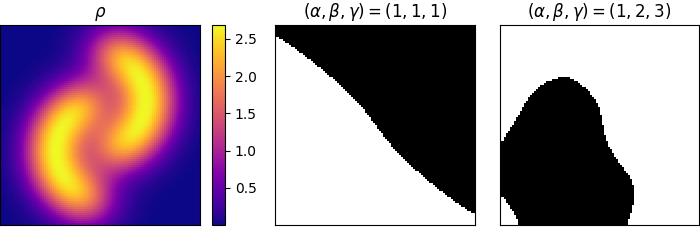
\includegraphics[width=4.5in]{images/moons.png}
}\hspace{0mm}
\subfloat[Noisy concentric circles]{
  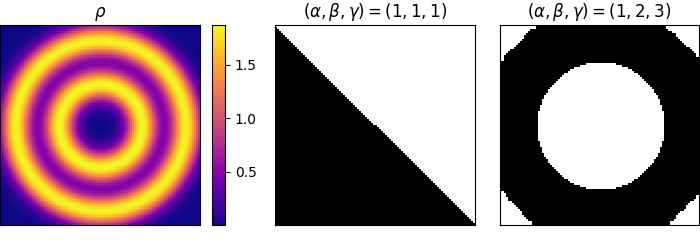
\includegraphics[width=4.5in]{images/circles.png}
}\hspace{0mm}
\subfloat[Long valley]{
  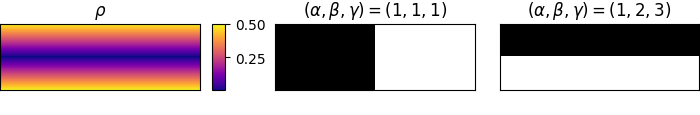
\includegraphics[width=4.5in]{images/trough.png}
}
\caption{
In each row, the first image shows the heat map of a fixed $\rho:\Omega\to\RR_>0$, the second and third images shows the set $\Omega_k$ returned by Algorithm \ref{alg:multiple_cuts} (displayed in black) for the choices $(\alpha,\beta,\gamma)$ of $(1,1,1)$ and $(1,2,3)$ respectively.
 }
\label{fig:alg}
\end{figure}


